\subsection{Übertragung von Daten}

Die Daten müssen auf beiden \ac{uC} ordnungsgemäß empfangen werden. Die Implementation unterscheidet sich hierbei stark. Der STM32 ermöglicht
die Nutzung seiner \ac{DMA}-Funktionalität, während auf dem ESP8266 eine Interruptbasierte Abfrage implementiert wird.

\subsubsection{STM32: Strukturvariable DMA\_STRUCT}

Aus Gründen der Übersichtlichkeit wurde für die Datenverarbeitung des STM32 eine Strukturvariable definiert, welche hiermit eingeführt wird.
Die Strukturvariable \lstinline!DMA_STRUCT! enthält mehrere weitere Variablen für Flags und Zähler.

\begin{lstlisting}[caption={\textit{DMA Strukturvariable}}]
typedef struct
{
    volatile uint8_t  t_flag;   
    uint8_t tx_flag;	
    volatile uint8_t av_flag;		
    uint16_t timer;             
    uint16_t prevCOUNT;      
    uint8_t data[DMA_BUF_SIZE];   
} DMA_STRUCT;
\end{lstlisting}

Die Flags \lstinline!t_flag! und \lstinline!tx_flag! dienen der Identifikation von Interrupts, welche durch im Falle von \lstinline!t_flag! durch ein
Timeout ausgelöst wurden oder im Falle von \lstinline!tx_flag! durch das erfolgreiche Senden von Daten. Die Variable \lstinline!timer! legt 
die Zeitkonstante für den Timeout fest, während \lstinline!prevCOUNT! einen Zähler speichert, der in \ref{subsub: Empfang} genauer erklärt wird.  

Das Flag \lstinline!av_flag! zeigt an, wenn neue Daten zur Verarbeitung verfügbar sind. Im Array \lstinline!data[]! werden die neuen Daten gespeichert.

\subsubsection{STM32: Konfiguration des UART}
Wichtig bei der Konfiguration des \acp{UART} ist das Format und die Baudrate. Wie in \ref{sec:Grundlagen} erklärt, wird der \ac{UART} im 8N1-Modus
konfiguriert. Dies entspricht einer Nachrichtenlänge von acht Bit und keiner Parität. Die Geschwindigkeit wird auf 115200 Baud festgelegt (siehe Abb. \ref{img: Parameter}). 

\begin{figure}[h]
  \centering
  \begin{subfigure}{0.45\textwidth}
      \centering
      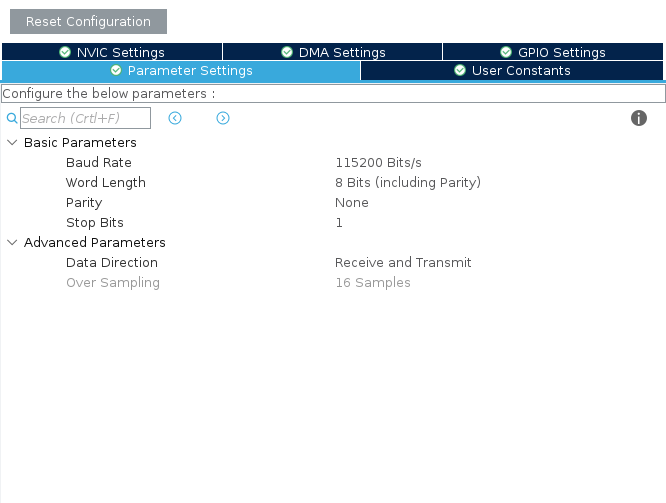
\includegraphics[width=\textwidth]{Pictures/parameter_uart.png}
      \caption{Baudrate,Format}
      \label{img: Parameter}
  \end{subfigure}
  %
  \begin{subfigure}{0.45\textwidth}
      \centering
      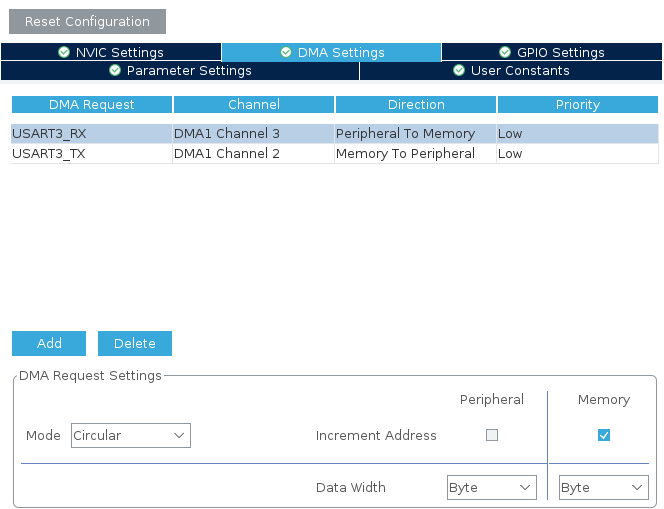
\includegraphics[width=\textwidth]{Pictures/dma_uart.png}
      \caption{DMA}
      \label{img: DMA}
  \end{subfigure}
  \caption{Konfiguration des \acp{UART}}
  \label{img: UART config}
\end{figure}

Um die Nutzung des \ac{UART} in Kombination mit \ac{DMA} zu ermöglichen, muss der globale Interrupt
aktiviert werden. Der \ac{DMA} wird so konfiguriert, dass empfangsseitig die Daten direkt zum Speicher übertragen werden, während senderseitig die Daten
direkt vom Speicher zum \ac{UART} weitergeleitet werden. Zudem wird der Empfang von Daten per \ac{DMA} als Ringbuffer umgesetzt (siehe Abb. \ref{img: DMA}).



\newpage
  \subsubsection{STM32: Idle Line Detection}
  \label{subsub: Idle}

  Es ist von großem Vorteil, zu erkennen, wenn keine Daten mehr Empfangen werden, um das schreiben von sinnlosen Daten in den Buffer zu vermeiden.
  Deshalb wird eine s.g. \textit{Idle Line Detection} implementiert, welche erkennt, sobald keine Daten mehr empfangen werden.



  Der STM32 bietet dafür einen Interrupt, welcher manuell aktiviert werden muss \citep{STM32_Ref}. Um den Interrupt zu aktivieren, muss während der Initialisierung
  der Interrupt aktiviert werden:
  \begin{lstlisting}
    __HAL_UART_ENABLE_IT(&huart3,UART_IT_IDLE);
  \end{lstlisting}
  
  Zudem muss in der Datei \lstinline!stm32f1xx_it.c! die Funktion 
  
  \lstinline!void USARTX_IRQHandler(void)! folgendermaßen erweitert werden:

  \begin{lstlisting}[caption={\textit{Idle Line Interrupt}}]
    if(__HAL_UART_GET_FLAG(&huartx,UART_FLAG_IDLE))
    {
        __HAL_UART_CLEAR_IDLEFLAG(&huartx);
        dma_info.timer = DMA_TIMEOUT_MS;
    }
  \end{lstlisting}

  Jedes mal, wenn ein Interrupt in Zusammenhang mit dem \ac{UART} ausgelöst wird, wird die Routine \lstinline!void USARTX_IRQHandler(void)! 
  aufgerufen und geprüft, ob es sich um ein Idle Line Interrupt handelt \citep{STM32_Ref}. 

  \smallskip

  Es ist allerdings nicht ausreichend, nur zu prüfen, ob der Interrupt aufgetreten ist - es kann durchaus vorkommen, dass es sich nur um eine
  kurze Unterbrechung in der Kommunikation handelt. Deshalb wird die Funktionalität um einen Timeout erweitert. Wenn der Interrupt auftritt, wird
  gleichzeitig die Strukturvariable \lstinline!dma_info.timer! mit einer definierten Zeitwert \lstinline!DMA_TIMEOUT_MS! geladen.

  \smallskip

  Um für zukünftige Erweiterungen keinen Timer zu blockieren, wird für den Timeout der Systick-Timer (\ref{subsub: Timer}) genutzt. Dieser implementiert eine Routine,
  welche im 10ms-Takt aufgerufen wird. Diese Routine ist ebenfalls in der Datei \lstinline!stm32fxx_it.c! zu finden und wird um folgenden Code
  erweitert:

  \begin{lstlisting}[caption={\textit{Systick Timer}}]
    if(dma_info.timer == 1)
    {
        dma_info.t_flag = 1;
        HAL_UART_RxCpltCallback(&huartx);
    }
    if(dma_info.timer) 
    { 
        --dma_info.timer; 
    }



  \end{lstlisting}
  
  Mittels dieser Erweiterung wird nun immer der Zähler des Timeouts dekrementiert, bis er eins erreicht. Wenn dies geschieht, wird ein Flag gesetzt
  und die Interruptroutine \lstinline!HAL\_UART\_RxCpltCallback(&huartx)! aufgerufen, in welcher anschließend der aufgetauchte Interrupt mittels des
  gesetzten Flags identifiziert und verarbeitet wird.
  
  \subsubsection{STM32: Empfangsinterrupt / DMA Circular Buffer}
  \label{subsub: Empfang}

  Während der Kommunikation mit \ac{UART} werden verschiedene Interrupts ausgelöst. Bei der Nutzung von \ac{DMA} werden Interrupts ausgelöst,
  wenn der Buffer halb oder ganz voll ist \citep{STM32_Ref}. Desweiteren wurde der \ac{uC} so konfiguriert, dass auch bei einem Idle Line Interrupt
  die entsprechende Interruptroutine aufgerufen wird \ref{subsub: Idle}.

  \smallskip

  Die Interruptroutinen sind nach der Generation von Code mittels CubeMX in der Datei \lstinline!stm32f1xx_hal.c! als \lstinline!__weak!
  definiert, werden also neu gesetzt sobald sie ohne das Keyword \lstinline!__weak! definiert werden \citep{HAL_Description}. 

  \smallskip

  In \lstinline!main.c! wird die Interruptroutine für den Empfang von Daten per \ac{UART} mit dem Namen 
  \begin{lstlisting}
    void HAL_UART_RxCpltCallback(UART_HandleTypeDef *huart)
  \end{lstlisting}
  initialisiert. 
  
  \smallskip

  Die Variablen \lstinline!pos!, \lstinline!start! und \lstinline!length! werden für den Ringbuffer benötigt. Die Variable \lstinline!currCount! speichert die aktuelle Position des
  Ringbuffers und wird über den Befehl
  
  \begin{lstlisting}
    __HAL_DMA_GET_COUNTER(huart->hdmarx)
  \end{lstlisting}
  beschrieben.

  \newpage

  Die Variable \lstinline!start! enthält die Startposition, ab welcher neue Daten im Ringbuffer enthalten sind. In der Variable \lstinline!length!
  ist die Länge der Daten gespeichert. Tritt ein Interrupt auf, weil der Empfangsbuffer voll ist, berechnet sich die Länge der empfangenen 
  Daten simpel durch folgenden Befehl:
  \begin{lstlisting}
    length = DMA_BUF_SIZE - start;
  \end{lstlisting}
  Es kann nun jedoch dazu kommen, dass nachdem der Buffer voll ist, ein Timeout-Interrupt ausgelöst wird. Um nun falsche Verarbeitung von 
  Daten zu verhindern, wird die aktuelle Position des Buffers auf die Größe des Buffers gesetzt.
  \begin{lstlisting}
    dma_info.prevCOUNT = DMA_BUF_SIZE;      
  \end{lstlisting}

  
  Wird nun ein Timeout-Interrupt ausgelöst, wird die Routine durch folgenden Code frühzeitig abgebrochen und das Flag rückgesetzt:
  \begin{lstlisting}[caption={\textit{Abbruch Timeoutinterrupt}}]
    if(dma_info.t_flag && currCOUNT == DMA_BUF_SIZE)
    {
        dma_info.t_flag = 0;
        return;
    }
  \end{lstlisting}

  \smallskip

  Tritt ein Interrupt auf, weil ein Timeout aufgetreten ist, muss unterschieden werden ob im Buffer bereits alte Daten liegen, welche ignoriert
  werden müssen oder ob der Buffer mit zu verarbeitenden Daten gefüllt ist. Folgender Code implementiert dies:

  \begin{lstlisting}[caption={\textit{Längenberechnung Timeout}}]
    if(dma_info.t_flag)
    {
    	if(dma_info.prevCOUNT < DMA_BUF_SIZE)
    	{
    		length = dma_info.prevCOUNT - currCOUNT;
    	}
    	else
    	{
  		length = DMA_BUF_SIZE - currCOUNT;
  	}

        dma_info.prevCOUNT = currCOUNT;
        dma_info.t_flag = 0;
    }
  \end{lstlisting}

  Wenn ein Timeout-Flag aufgetreten ist, wird geprüft ob der alte Zähler des Ringbuffers kleiner als die Buffergröße ist. Ist dies der Fall, berechnet
  sich die Länge der Daten durch die Differenz zwischen dem alten und dem neuen Zählerwert, da noch alte Daten im Buffer gespeichert sind.
  
  Wenn keine alten Daten im Buffer gespeichert sind, berechnet sich die Länge durch die Differenz zwischen der Buffergröße und der aktuellen Zählerposition.

  \smallskip

  Im Anschluss wird der Zählerwert des \ac{DMA} übergeben und das Timeout-Flag rückgesetzt.

  \smallskip

  Die Startposition der neuen Daten berechnet sich ähnlich. Ist der alte Zähler des Ringbuffers kleiner als die Buffergröße, ist die Startposition
  die Differenz zwischen der Buffergröße und des alten Zählerwerts. Wenn nicht, ist die Startposition gleich null.

  \begin{lstlisting}[caption={\textit{Berechnung Startposition}}]
    if(dma_info.prevCOUNT<DMA_BUF_SIZE)
    {
    	start = (DMA_BUF_SIZE-dma_info.prevCOUNT);
    }
    else
    {
    	start = 0;
    }  
  \end{lstlisting}

  \smallskip

  Mit Hilfe der berechneten Werten für die Startposition und die Länge der empfangenen Daten werden diese Daten zu guter Letzt in ein dediziertes
  Array zur Weiterverarbeitung kopiert und ein Flag gesetzt, welches anzeigt, dass neue Daten vorhanden sind:
  
  \begin{lstlisting}[caption={\textit{Kopieren neuer Daten}}]
    for(uint16_t i=0,pos=start; i<length; ++i,++pos)
    {
        dma_info.data[i] = dma_rx_buf[pos];
    }
    dma_info.av_flag = 1;
  \end{lstlisting}

  Mit den Informationen über das Protokoll aus \ref{subsub: Datenformat} lassen sich nun aus dem Array in dem die angekommenen Daten gespeichert wurden, die Telegramme extrahieren.

\subsubsection{STM32: Überprüfen der Daten}

Die empfangenen Daten müssen auf ihre Integrität getestet werden. Dazu wurde in \ref{subsub: CRC16} das Konzept der zyklischen Redundanzprüfung eingeführt.

\smallskip

Um die empfangenen Daten zu prüfen, wird das Array welches die Daten enthält der Funktion 
\begin{lstlisting}
  uint8_t data_check(uint8_t *dat)
\end{lstlisting}
übergeben. Diese Funktion extrahiert die CRC-Prüfsumme sowie die Länge der Nachricht und validiert diese. Wenn die zyklische Redundanzprüfung erfolgreich
ist, wird die Länge der Nachricht übergeben. Wenn sie fehlschlägt, wird eine null zurückgegeben.

\newpage

\subsubsection{STM32: Versenden von Daten}

Das Versenden von Daten geschieht mittels der Funktion \citep{HAL_Description}
\begin{lstlisting}
  HAL_StatusTypeDef HAL_UART_Transmit_DMA(UART_HandleTypeDef *huart,
  uint8_t *pData, uint16_t Size)
\end{lstlisting}

Es werden der Handler, welcher dem genutzten \ac{UART} zugeordnet ist, übergeben, sowie den zu übertragenden Buffer und die Länge des Buffers. 

\smallskip

Wichtig bei der Nutzung der Funktion ist das Abwarten, ob die Daten versendet wurden. Wird die Funktion zu früh ein zweites mal aufgerufen, werden die Daten
welche sich gerade im Sendebuffer befinden überschrieben \citep{HAL_Description}. Eine Prüfung ob die Funktion \lstinline!HAL_OK! zurückgibt, ist nicht ausreichend,
da dies bereits geschieht bevor alle Daten übertragen wurden.

\smallskip

Ähnlich wie bei dem Empfang von Daten gibt es auch bei der Versendung von Daten einen Interrupt, sobald die Daten erfolgreich versendet wurden \citep{HAL_Description}. Mittels des
Flags \lstinline!uart_info.tx_flag!, welches innerhalb der zugehörigen Interruptroutine gesetzt wird, wird die Vollendung der Übertragung kontrolliert.

\smallskip

Dieser zusammenhang wird in folgender Funktion umgesetzt:

\begin{lstlisting}[caption={\textit{Warten auf Versand}}]
  void tx_wait(DMA_STRUCT * dma)
  {
    while(!dma->tx_flag);						
    dma->tx_flag=0;								
  }
\end{lstlisting}

Es wird die DMA-Strukturvariable übergeben und gewartet, bis das Flag in der Interruptroutine gesetzt wurde. Sobald dies geschehen ist, wird es rückgesetzt - neue
Daten können versendet werden.




\subsubsection{ESP8266: Empfang und Überprüfung der Daten}

Die Implementation für den Empfang von Daten ist simpler gehalten, primär auf Grund des vereinfachenden Arduino-Frameworks. Die Funktion \lstinline!void receive()!
implementiert die Funktionalität des Datenempfangs. Ähnlich wie bei der Implementation des STM32, wird hier ein Timeout genutzt, jedoch auf fortgeschrittene 
Technologien wie \ac{DMA} verzichtet.

\smallskip

Folgende Variablen werden innerhalb der Funktion genutzt:

\begin{lstlisting}[caption={\textit{Variablen receive()}}]
  static uint16_t count = 0;
  static bool InProg = false;
  static uint8_t len= 0;
  uint16_t crc_calc;
  static uint32_t tim;  
\end{lstlisting}

Die Variable \lstinline!count! zählt die Anzahl der empfangenen Bytes, während \lstinline!InProg! anzeigt, dass zurzeit Daten empfangen werden. Zudem speichert
\lstinline!len! die Länge der empfangenen Nachricht, während \lstinline!tim! die Zählervariable für den Timeout implementiert. Um das Ergebnis der zyklischen
Redundanzprüfung zu speichern, wird \lstinline!crc_calc! genutzt.

\smallskip

Desweiteren werden weitere globale Variablen benötigt:

\begin{lstlisting}[caption={\textit{Globale Variablen receive()}}]
  uint8_t receivedChars[BUF_SIZE];   
  bool newData = false
\end{lstlisting}

Das Array \lstinline!receivedChars[]! speichert die empfangenen Daten. Durch die Variable \lstinline!newData! wird die Verfügbarkeit von neuen Daten angezeigt.

\smallskip

Die Implementation bedient sich diversen Befehlen aus dem Arduino-Framework \citep{ArduinoRef}:

\begin{itemize}
  \item \lstinline!Serial.available()! - Prüfen ob neue Daten vorhande sind
  \item \lstinline!Serial.read()! - Einlesen eines Bytes 
  \item \lstinline!millis()! - Auslesen der verstrichenen Zeit in ms
\end{itemize}

Um Funktionen welche im Zusammenhang mit dem \ac{UART} stehen, nutzen zu können, muss dieser während des Starts des \ac{uC} mit der Baudrate initialisiert werden \citep{ArduinoRef}:
\begin{lstlisting}[caption={\textit{Initialiserung UART}}]
  Serial.begin(BAUD);
\end{lstlisting}

Die Funktion \lstinline!void receive()! wird kontinuierlich in der Main-Loop aufgerufen.

\smallskip


Mittels einer While-Schleife wird geprüft, ob Daten verfügbar sind und ob Daten, welche zuvor empfangen wurden, verarbeitet werden müssen. Wenn diese Bedingung erfüllt
ist, wird der Zähler des Timers auf den aktuellen wert aktualisiert und ein Byte eingelesen. 

\begin{lstlisting}[caption={\textit{Prüfen auf neue Daten}}]
  while (Serial.available() > 0 && newData == false)
  {
      tim = millis();
      receivedChars[count] = Serial.read();
\end{lstlisting}

Nach jedem durchlauf der kompletten While-Schleife wird der Zähler \lstinline!count! inkrementiert, um das nächste Zeichen einzulesen.

\newpage

Wird ein Start-Zeichen im empfangenen Telegramm (siehe \ref{subsub: Datenformat}) erkannt, wird die Variable \lstinline!InProg! gesetzt, um die weitere Verarbeitung
zu erlauben:

\begin{lstlisting}[caption={\textit{Erkennung Start-Marker}}]
  if (receivedChars[count] == START_MARKER)
  {
    InProg = true;
  }
\end{lstlisting}

Auf Basis der aktuellen Anzahl an eingelesenen Zeichen und dem gesetzten Flag wird nun das einlesen der Längeninformation ermöglicht:

\begin{lstlisting}
  if(InProg == true && count == 2)
  {
    len = (receivedChars[count]-OFF_ASCII)
    +((receivedChars[count-1]-OFF_ASCII)*10);
  }
\end{lstlisting}

Die Länge muss dafür zu einer Integervariable konvertiert werden. Dies geschieht durch die Subtraktion des Offsets (48) und dem Zusammenführen der verschiedenen Stellen.

\smallskip

Basierend auf der eingelesenen Länge der Nachricht, kann festgestellt werden, wann die CRC-Prüfsumme eingelesen wurde \ref{subsub: Datenformat}. Mittels der Prüfsumme
wird dann die zyklische Redundanzprüfung durchgeführt und bei Erfolg die Variablen der Funktion rückgesetzt und das Flag zum anzeigen von neuen Daten gesetzt. War die Prüfung
nicht erfolgreich, wird das Flag nicht gesetzt.

\begin{lstlisting}[caption={\textit{Zyklsiche Redundanzprüfung}}]
  if(InProg == true && count == len+4)
      {
        crc_calc = CRC16_buf(receivedChars,count+1); 
        if(crc_calc == 0)
        {
          length_pub = len;
          InProg = false; 
          newData = true; 
          len = 0;        
          count = 0;      
          return;
        }
        else
        {
          InProg = false;  
          newData = false; 
          len = 0;         
          count = 0;        
          return;         
        }
\end{lstlisting}

Da der Zähler \lstinline!count! am Ende der While-Schleife inkrementiert wird, muss der Funktion der zyklischen Redundanzprüfung \lstinline!count+1! übergeben werden.

\smallskip

Bevor jedoch die soeben erklärte While-Schleife aufgerufen wird, wird geprüft ob ein Timeout eingetreten ist. Diese Überprüfung bedient sich der gespeicherten Zeit und 
der aktuellen Zeit sowie dem Flag \lstinline!InProg!, welches anzeigt, ob eine Transaktion im Gange ist. Ist die Differenz zwischen aktueller Zeit und der gespeicherten Zeit
zu groß und das Flag gesetzt, werden die Variablen \lstinline!count! und \lstinline!InProg! rückgesetzt und das Einlesen abgebrochen:

\begin{lstlisting}[caption={\textit{Abbruch durch Timeout}}]
  if (InProg == true && (millis() - tim > TIMEOUT))
  {
    count = 0;
    InProg = false;
  }
\end{lstlisting}